\documentclass[12pt, a4paper]{article}

\usepackage[utf8]{inputenc}
\usepackage{geometry}
\geometry{margin=1in}
\usepackage{graphicx}
\usepackage{hyperref}
\usepackage{booktabs}
\usepackage{amsmath}
\usepackage{float}
\usepackage{caption}
\usepackage{subcaption}

\title{Multi-Objective Optimization for Fairness and Complexity in Machine Learning}
\author{Daksh Rajesh \and Mohammad Owais}
\date{\today}

\begin{document}

\maketitle

\begin{abstract}
Our report describes a methodical approach towards implementing MOO for prediction models using COMPAS dataset. Through the use of NSGA-II algorithm (from the Python library Pymoo) along with the NSGAIISampler in Optuna, we simultaneously maximize prediction accuracy, minimize demographic parity, and the complexity of our model. This method allows for revealing tradeoffs between these three goals and ultimately finding an optimal compromise.
\end{abstract}

\section{Introduction}
Modern machine learning models are often optimized solely for predictive performance (e.g., accuracy, AUC). However, in high-stakes domains such as criminal justice, evaluating models across a single dimension is insufficient. Models must also exhibit fairness across sensitive demographic groups and remain interpretable and computationally lightweight. This project explores the use of evolutionary algorithms to discover optimal trade-offs between these competing priorities, mapping out a multi-dimensional Pareto frontier.

\section{Problem Statement and Objectives}
The primary problem addressed in this study is the simultaneous optimization of a machine learning pipeline across three inherently conflicting objectives. In standard optimization, improving fairness often degrades accuracy, while increasing accuracy often requires highly complex (and less interpretable) models.

Our multi-objective formulation seeks to minimize the following three objective functions:

\begin{enumerate}
    \item \textbf{Minimize $(1 - \text{Balanced Accuracy})$:} 
    Balanced accuracy is used instead of standard accuracy to account for class imbalances in the COMPAS dataset. Maximizing balanced accuracy corresponds to minimizing its complement.
    
    \item \textbf{Minimize Demographic Parity (DP) Violation:} 
    Fairness is quantified as the absolute difference in the positive prediction rate (recidivism prediction) between the unprivileged group (African-American) and the privileged group (Caucasian).
    \[
    f_2 = |P(\hat{Y}=1 \mid A=\text{African-American}) - P(\hat{Y}=1 \mid A=\text{Caucasian})|
    \]
    
    \item \textbf{Minimize Model Complexity:} 
    We define a normalized metric $\in [0, 1]$ representing the computational and structural complexity of the chosen model. Logistic Regression is penalized linearly by its regularization strength, while tree-based models (Random Forest, XGBoost) are penalized based on their number of estimators and maximum tree depth. This objective acts as a proxy for interpretability and deployment cost.
\end{enumerate}

These three objectives are intrinsically conflicting. Achieving zero DP violation often requires severely degrading predictive accuracy, and reaching peak accuracy typically demands high model complexity.

\section{Methodologies}
To navigate this complex search space consisting of mixed-variable hyperparameters (model type, regularization, learning rate, tree depth, etc.), we employed two distinct NSGA-II based methodologies.

\subsection{Method 1: NSGA-II via Pymoo (\texttt{moo\_nsga2\_pymoo.py})}
The first methodology utilizes \texttt{pymoo}, a specialized library for multi-objective optimization. 
\begin{itemize}
    \item \textbf{Core Components:}
    \begin{itemize}
        \item \texttt{load\_and\_preprocess\_compas()}: Handles the loading and standardized ProPublica filtering of the dataset.
        \item \texttt{compute\_fairness\_metrics()}: Calculates the Demographic Parity violation across the sensitive groups.
        \item \texttt{compute\_model\_complexity()}: Evaluates the normalized structural complexity of the generated models.
        \item \texttt{FairnessMOOProblem}: A custom class inheriting from \texttt{pymoo.core.problem.Problem} that formally defines the 7 decision variables (including continuous variables like learning rate and discrete variables like model type) and the 3 objectives.
    \end{itemize}
    \item \textbf{Execution:} The algorithm was configured with a population size of 150 and run for 150 generations (evaluating roughly 22,500 candidate models) using Simulated Binary Crossover (SBX) and Polynomial Mutation (PM).
\end{itemize}

\pagebreak

\subsection{Method 2: Optuna NSGA-II Sampler (\texttt{moo\_optuna\_comparison.py})}
The second methodology relies on Optuna, a highly efficient hyperparameter optimization framework utilizing its native \texttt{NSGAIISampler}.
\begin{itemize}
    \item \textbf{Core Components:}
    \begin{itemize}
        \item While reusing the data loading and complexity metric functions, this script defines a unified \texttt{optuna\_objective(trial)} function.
        \item The objective function utilizes Optuna's \texttt{trial.suggest\_categorical},\newline
        \texttt{trial.suggest\_float}, and \texttt{trial.suggest\_int} APIs to dynamically sample the search space.
        \item \texttt{evaluate\_optuna\_pareto()}: Extracts the best trials forming the Pareto front and performs out-of-sample evaluation on the test set.
    \end{itemize}
    \item \textbf{Execution:} The study was executed for 2,500 multi-objective trials. While Optuna is generally more sample-efficient through its Bayesian-guided approach, Pymoo provides more rigorous population-based evolutionary dynamics.
\end{itemize}

\section{Results and Visualizations}
The optimization successfully identified dense Pareto frontiers for both methodologies. The results were parsed to visualize the exact dynamics of the trade-offs.

\subsection{Algorithm Comparison and Trade-offs}
Figure \ref{fig:aggregate} illustrates the global performance and interactions of the objectives. 

\begin{figure}[H]
    \centering
    \begin{subfigure}[b]{0.45\textwidth}
        \centering
        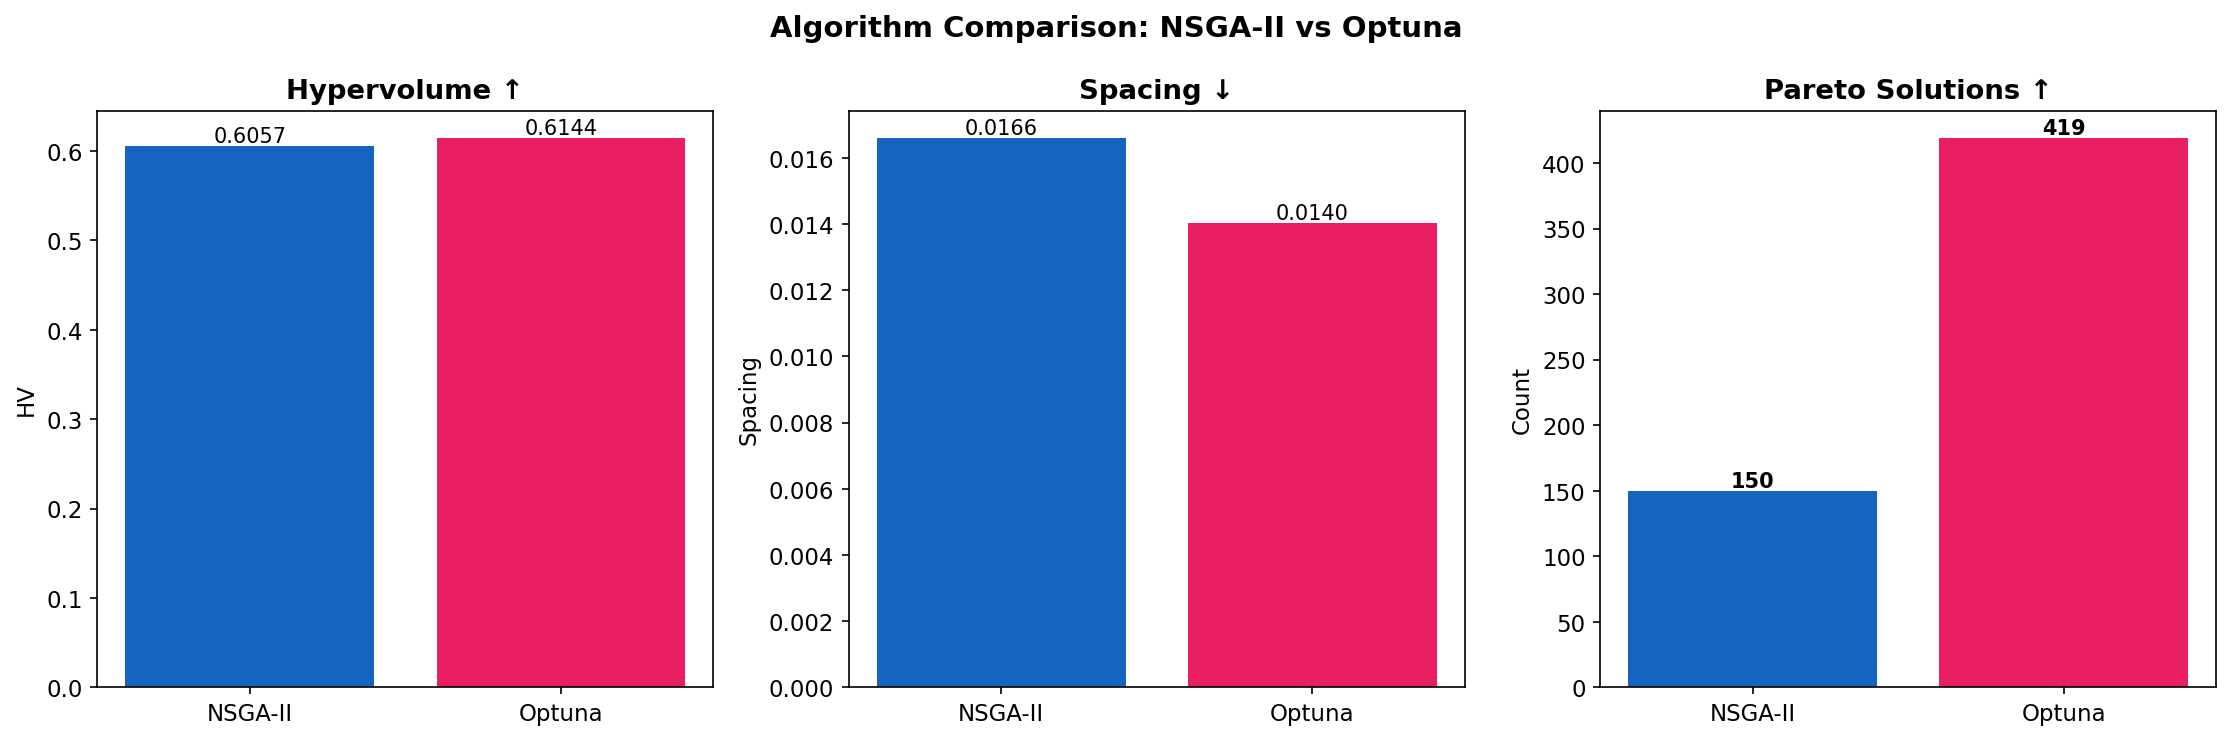
\includegraphics[width=\textwidth]{results/algorithm_comparison.png}
        \caption{Algorithm Comparison (Hypervolume \& Spacing)}
    \end{subfigure}
    \hfill
    \begin{subfigure}[b]{0.45\textwidth}
        \centering
        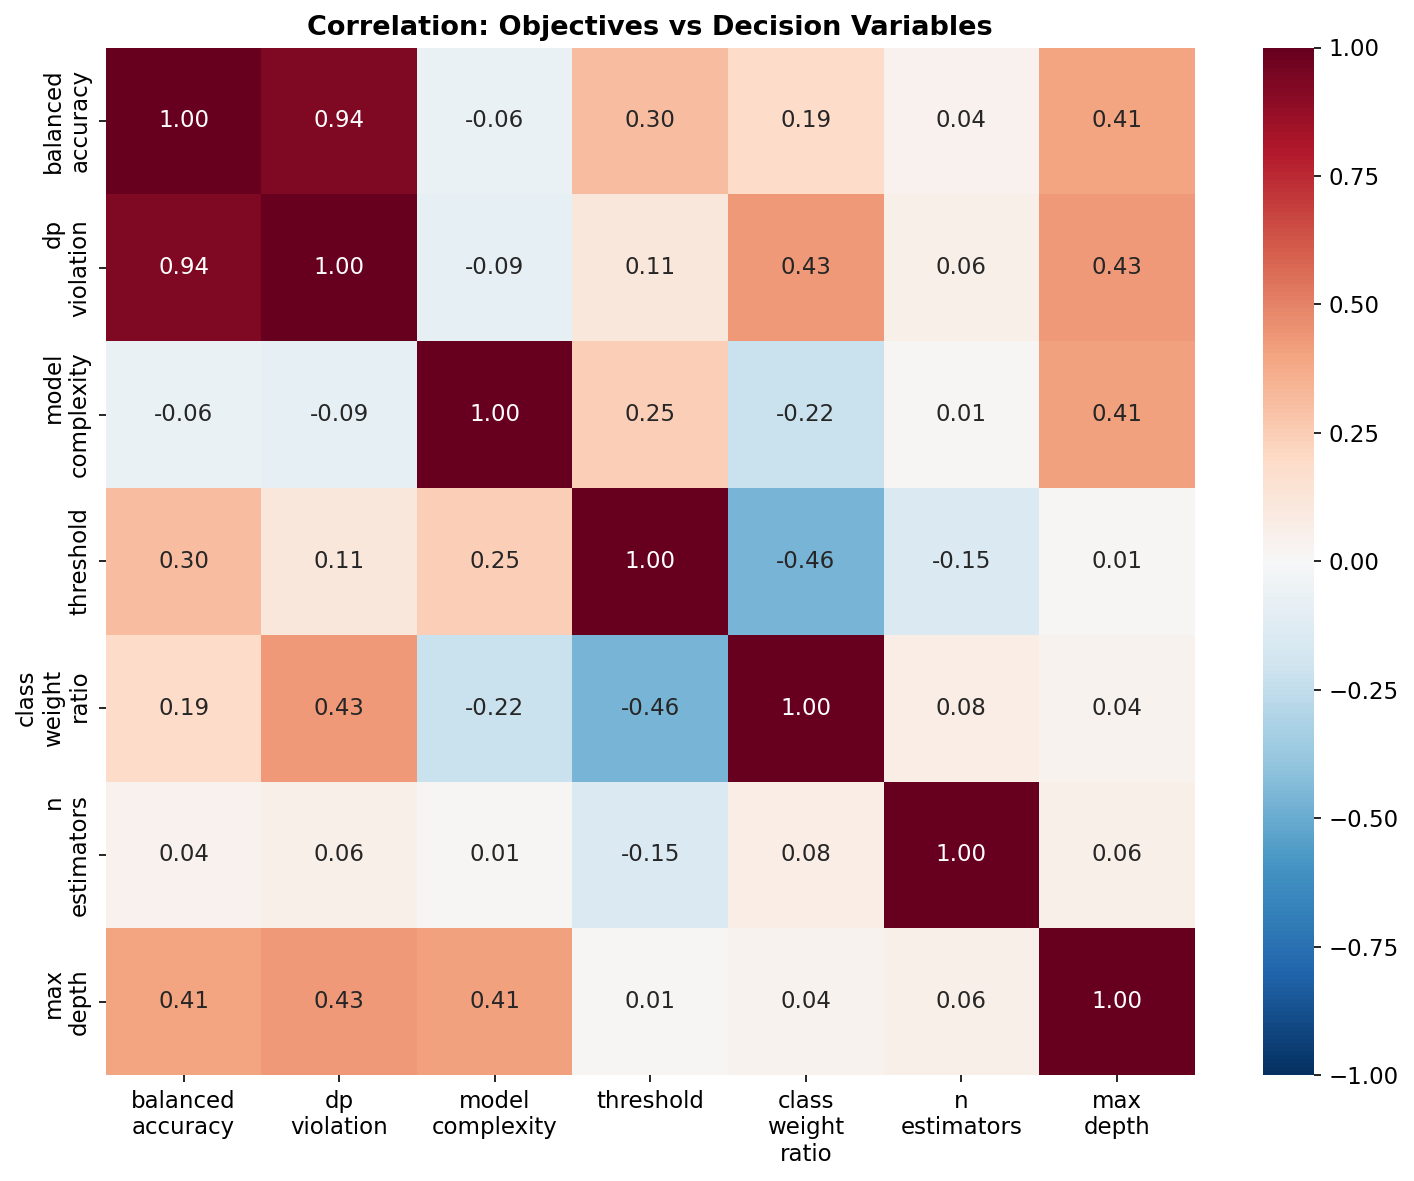
\includegraphics[width=\textwidth]{results/tradeoff_heatmap.png}
        \caption{Objective Trade-off Heatmap}
    \end{subfigure}
    \caption{Aggregate summaries detailing algorithm performance and inter-objective correlations.}
    \label{fig:aggregate}
\end{figure}

\subsection{Pareto Projections}
To understand how model complexity affects fairness and accuracy, we project the 3D Pareto frontier into 2D spaces. In these visualizations, sub-optimal (dominated) solutions are plotted as a dimmed background cloud, while the optimal frontier is boldly highlighted.

\begin{figure}[H]
    \centering
    \begin{subfigure}[b]{0.32\textwidth}
        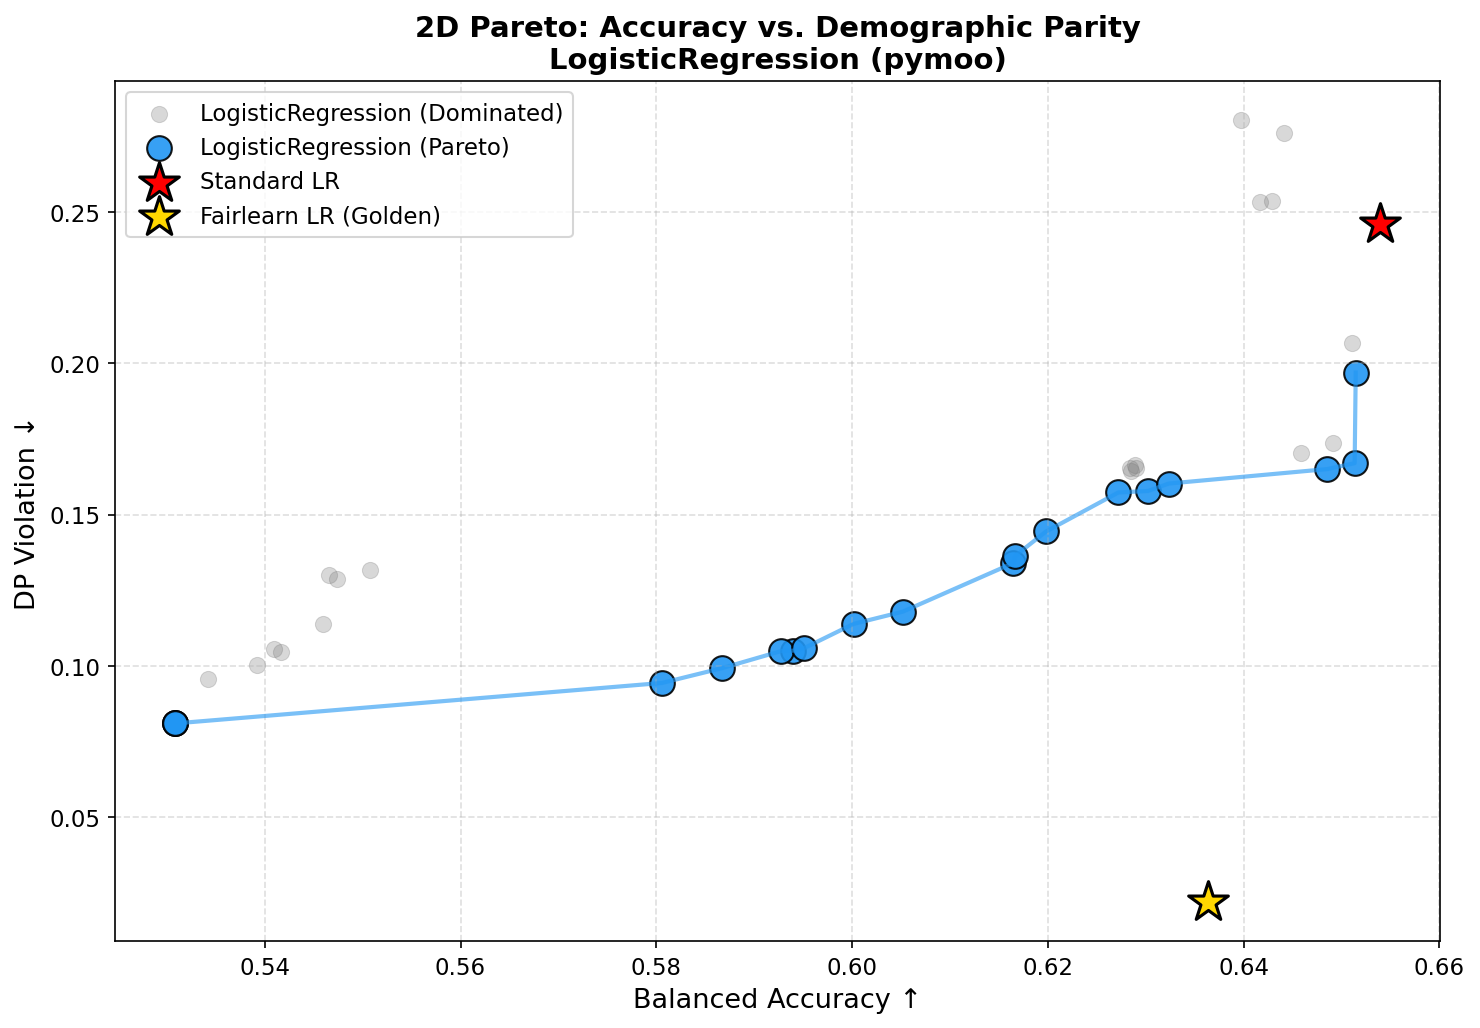
\includegraphics[width=\textwidth]{results/pymoo/LogisticRegression/pareto_2d_balanced_accuracy_vs_dp_violation.png}
        \caption{Logistic Regression}
    \end{subfigure}
    \hfill
    \begin{subfigure}[b]{0.32\textwidth}
        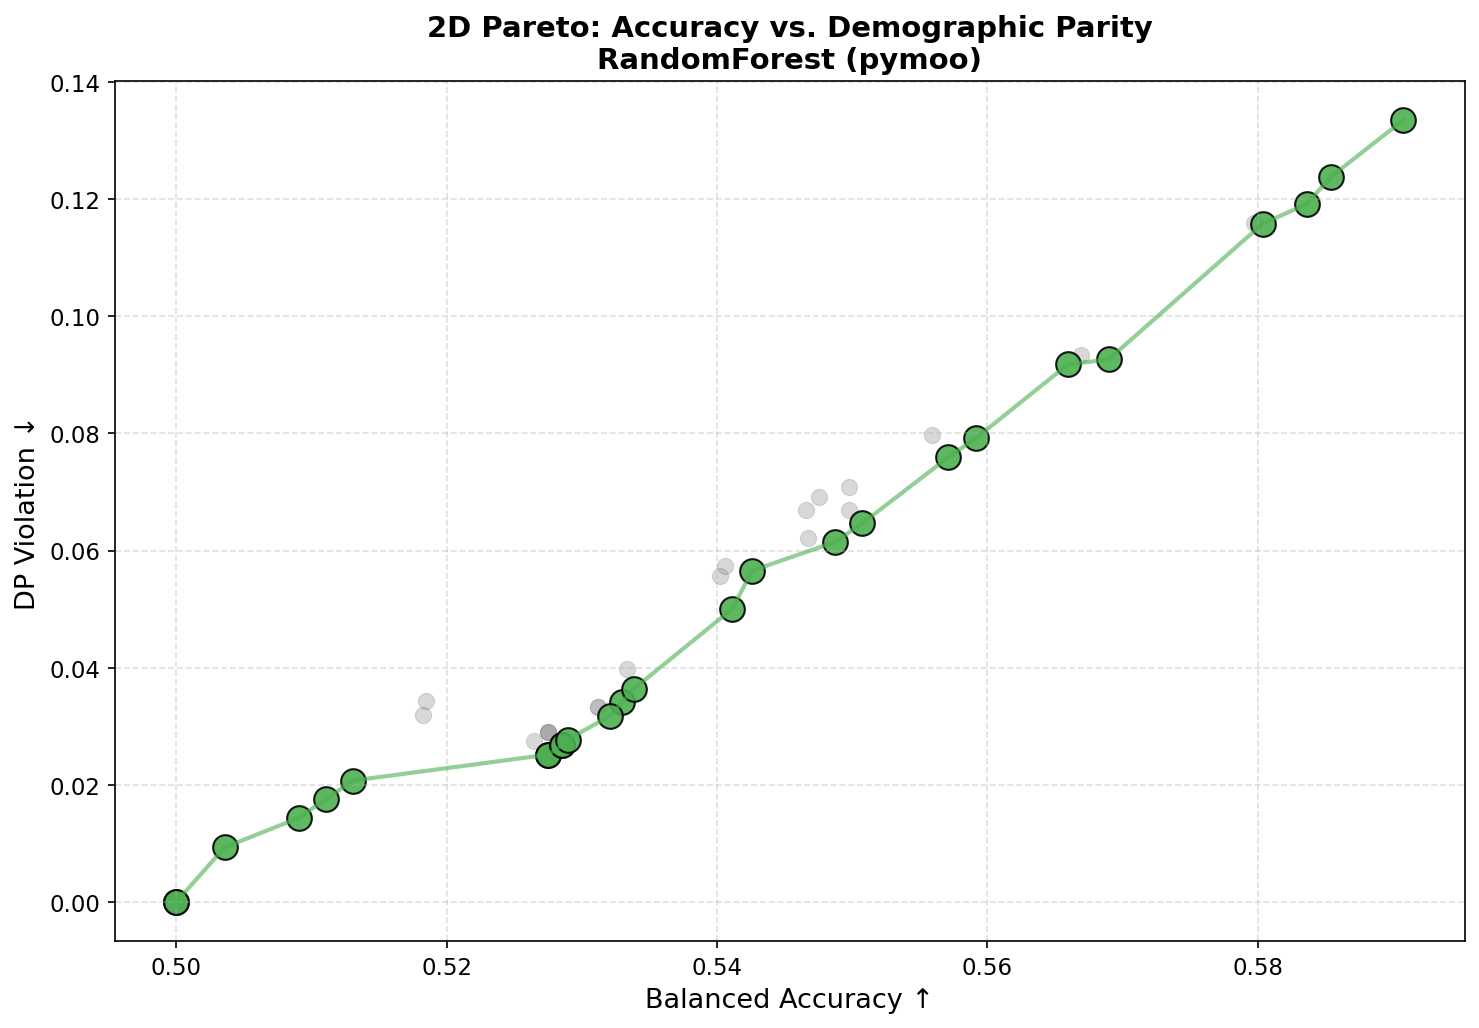
\includegraphics[width=\textwidth]{results/pymoo/RandomForest/pareto_2d_balanced_accuracy_vs_dp_violation.png}
        \caption{Random Forest}
    \end{subfigure}
    \hfill
    \begin{subfigure}[b]{0.32\textwidth}
        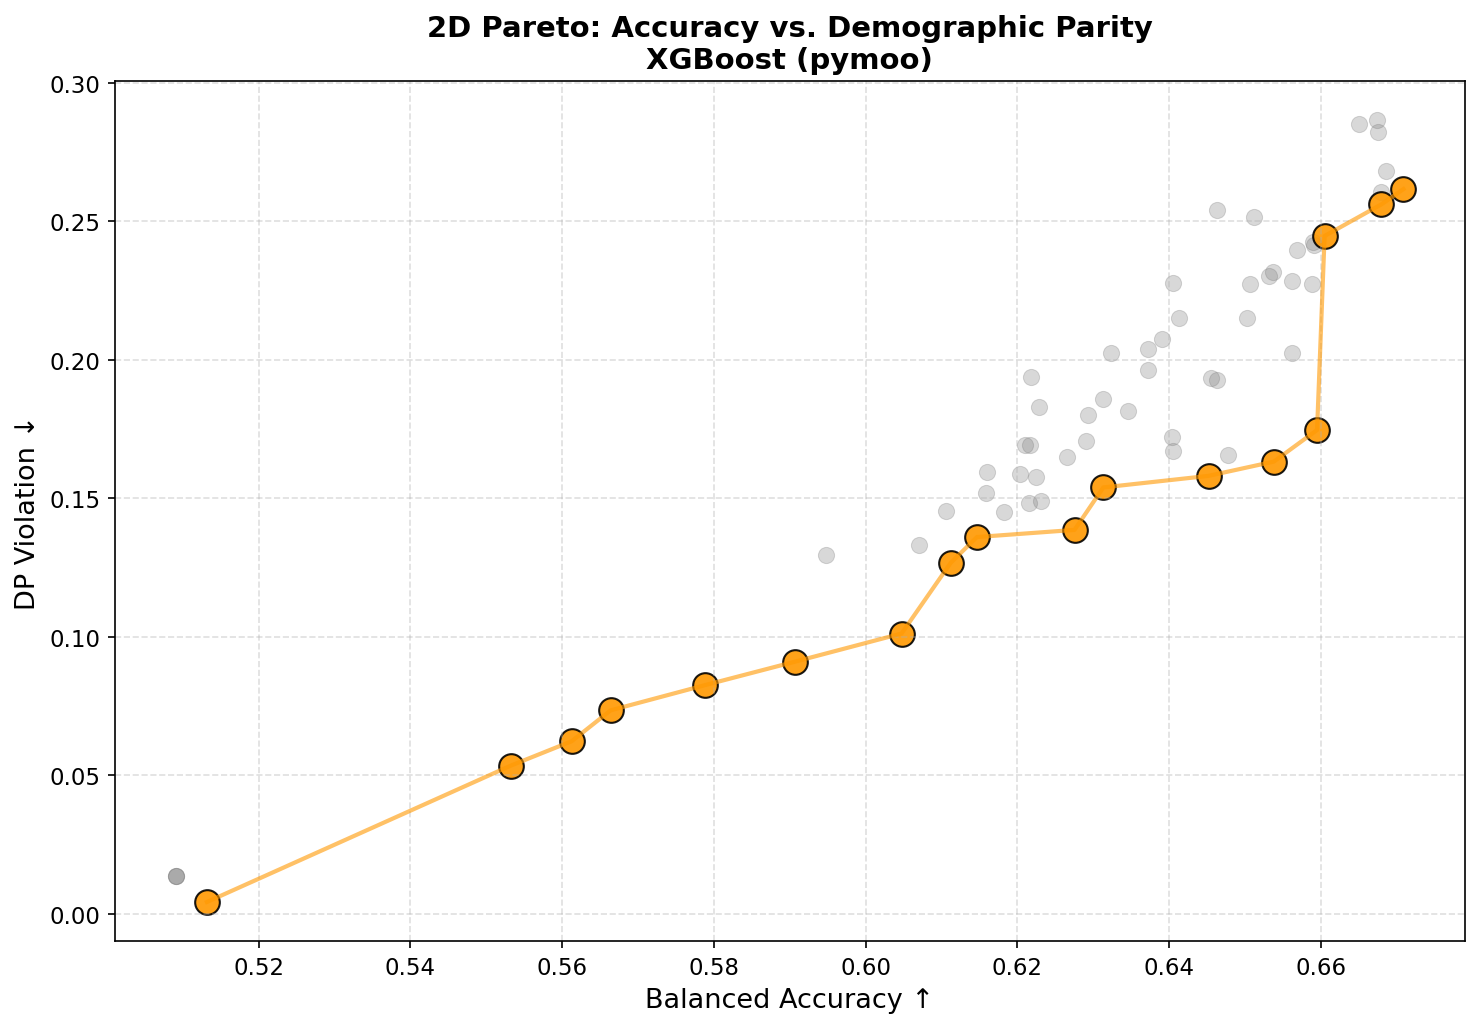
\includegraphics[width=\textwidth]{results/pymoo/XGBoost/pareto_2d_balanced_accuracy_vs_dp_violation.png}
        \caption{XGBoost}
    \end{subfigure}
    \caption{Pymoo NSGA-II: Balanced Accuracy vs. Demographic Parity Violation across three model types.}
    \label{fig:pymoo_acc_dp}
\end{figure}

\begin{figure}[H]
    \centering
    \begin{subfigure}[b]{0.32\textwidth}
        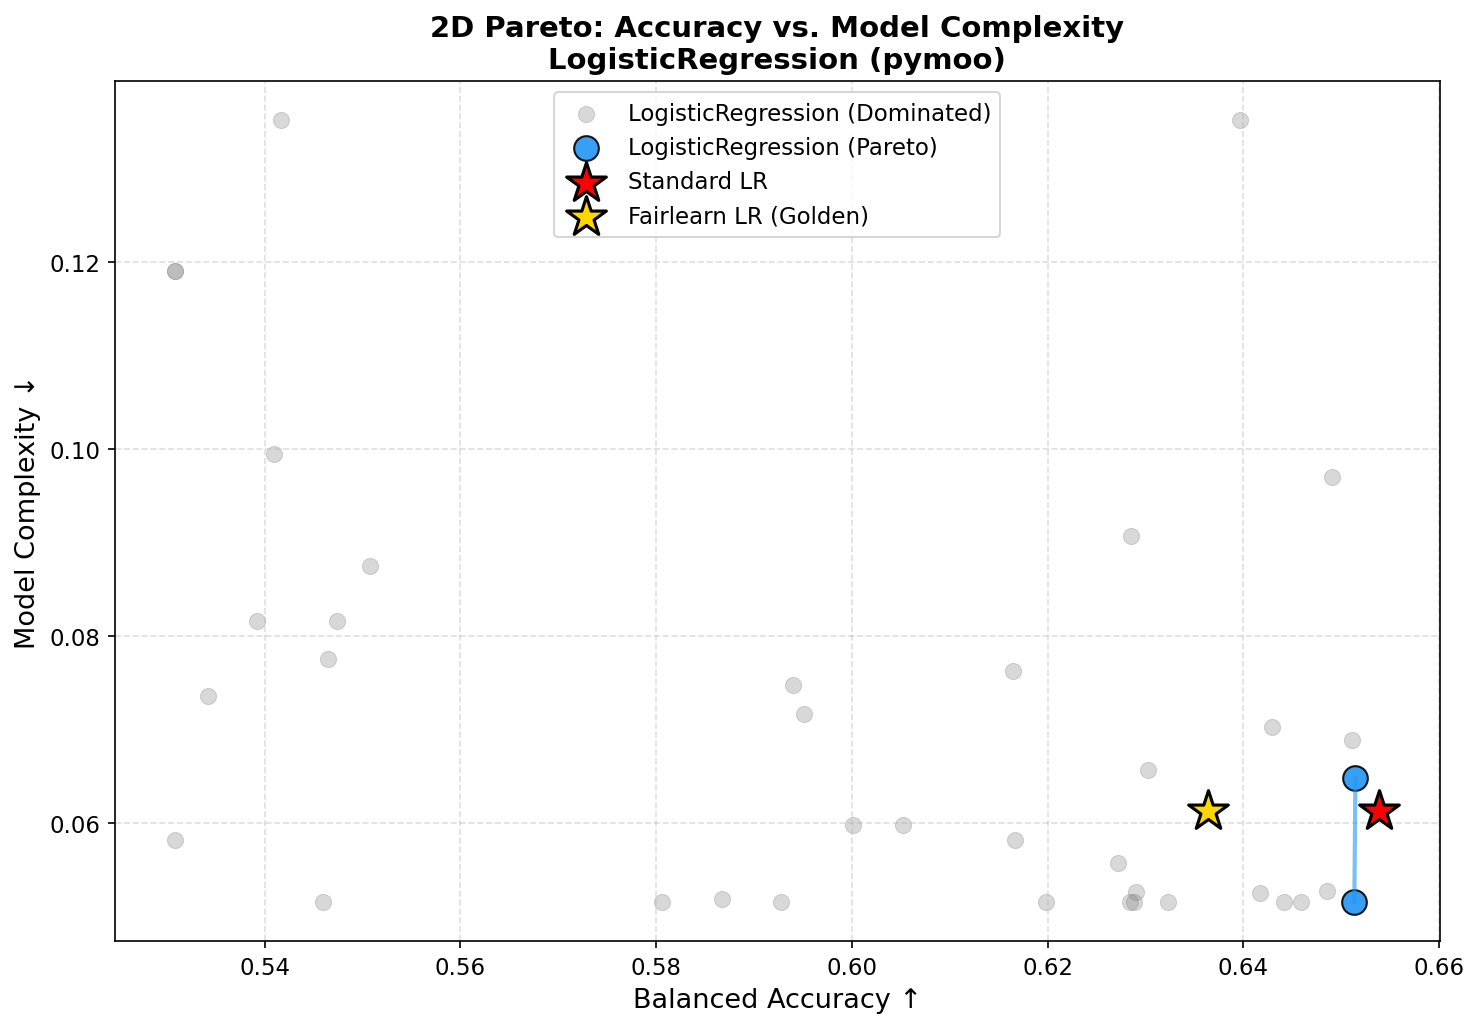
\includegraphics[width=\textwidth]{results/pymoo/LogisticRegression/pareto_2d_balanced_accuracy_vs_model_complexity.png}
        \caption{Logistic Regression}
    \end{subfigure}
    \hfill
    \begin{subfigure}[b]{0.32\textwidth}
        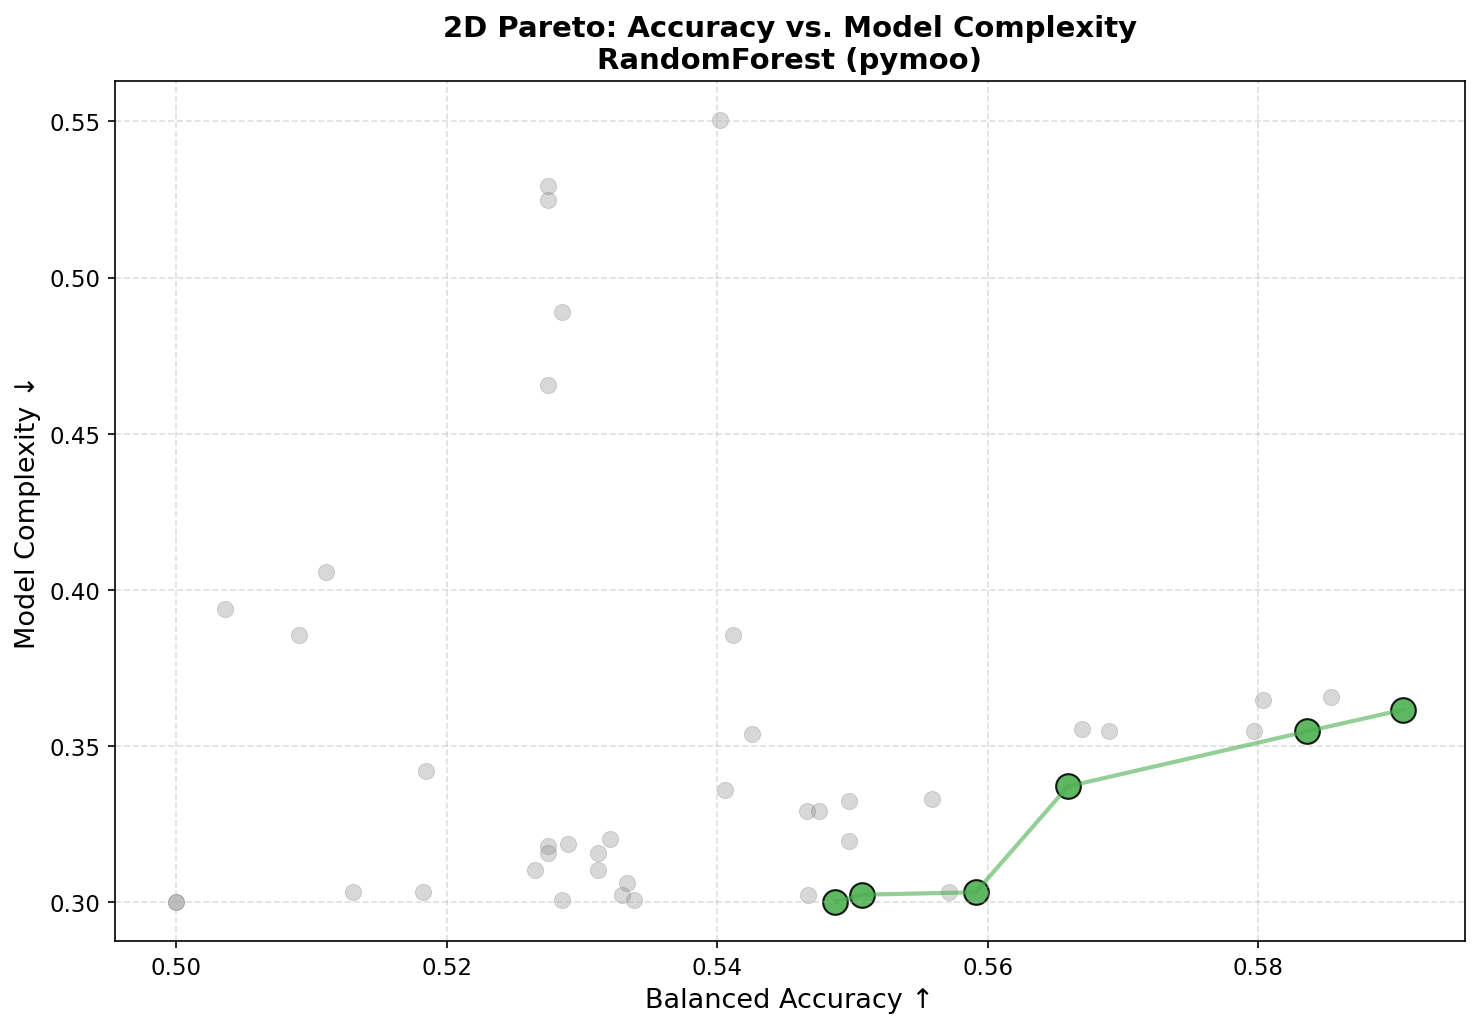
\includegraphics[width=\textwidth]{results/pymoo/RandomForest/pareto_2d_balanced_accuracy_vs_model_complexity.png}
        \caption{Random Forest}
    \end{subfigure}
    \hfill
    \begin{subfigure}[b]{0.32\textwidth}
        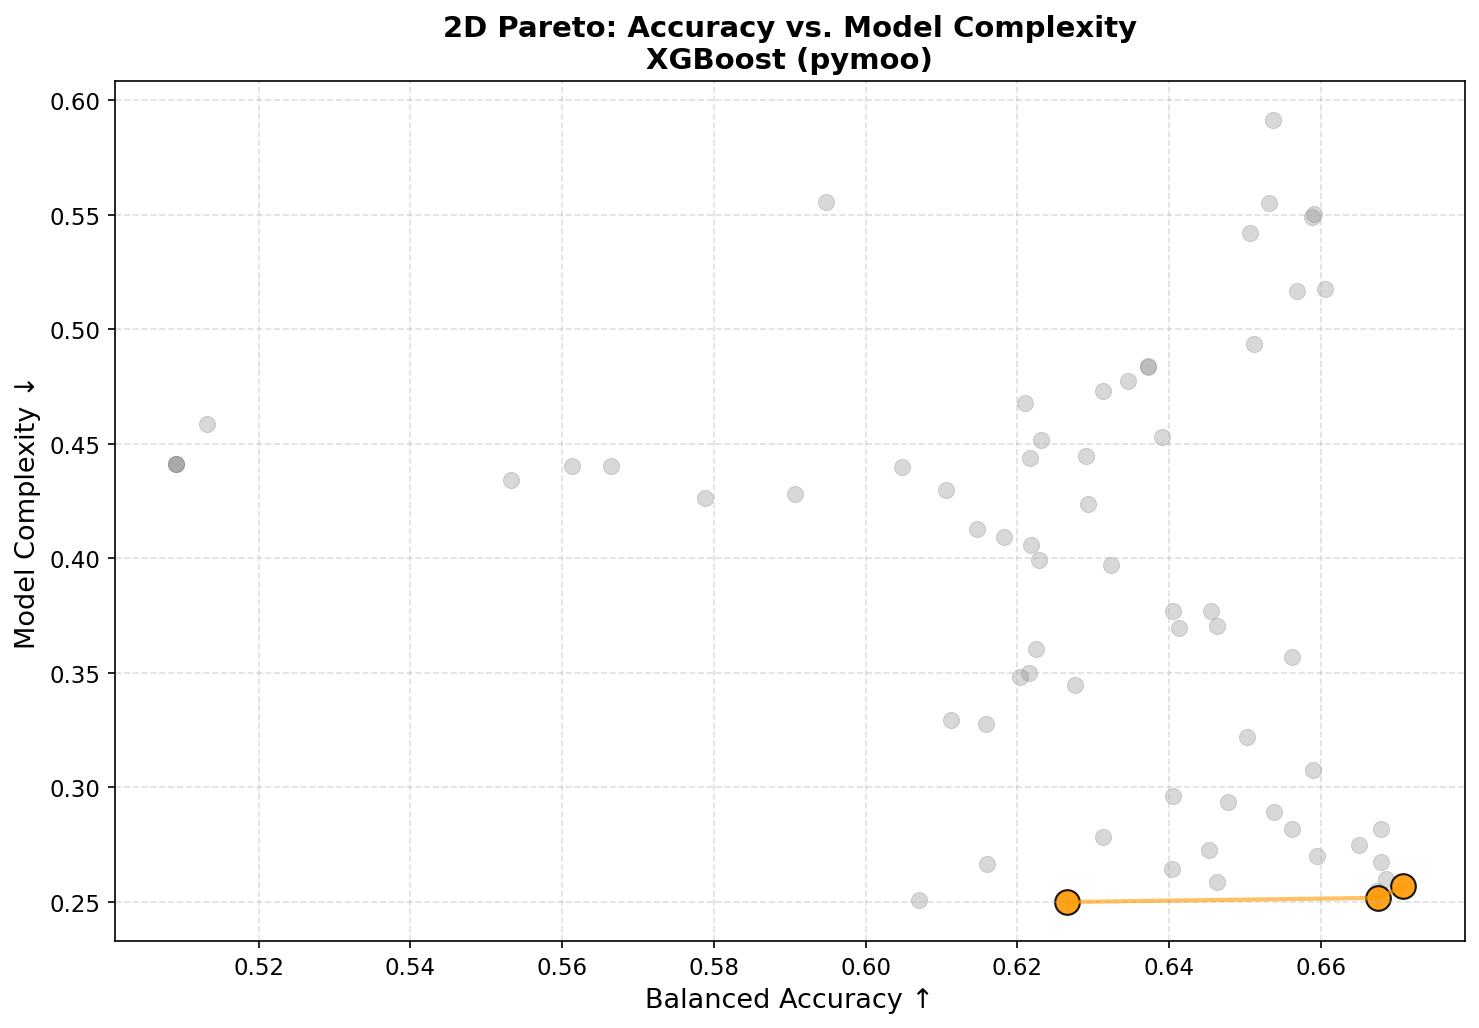
\includegraphics[width=\textwidth]{results/pymoo/XGBoost/pareto_2d_balanced_accuracy_vs_model_complexity.png}
        \caption{XGBoost}
    \end{subfigure}
    \caption{Pymoo NSGA-II: Balanced Accuracy vs. Model Complexity across three model types.}
    \label{fig:pymoo_acc_comp}
\end{figure}

\begin{figure}[H]
    \centering
    \begin{subfigure}[b]{0.32\textwidth}
        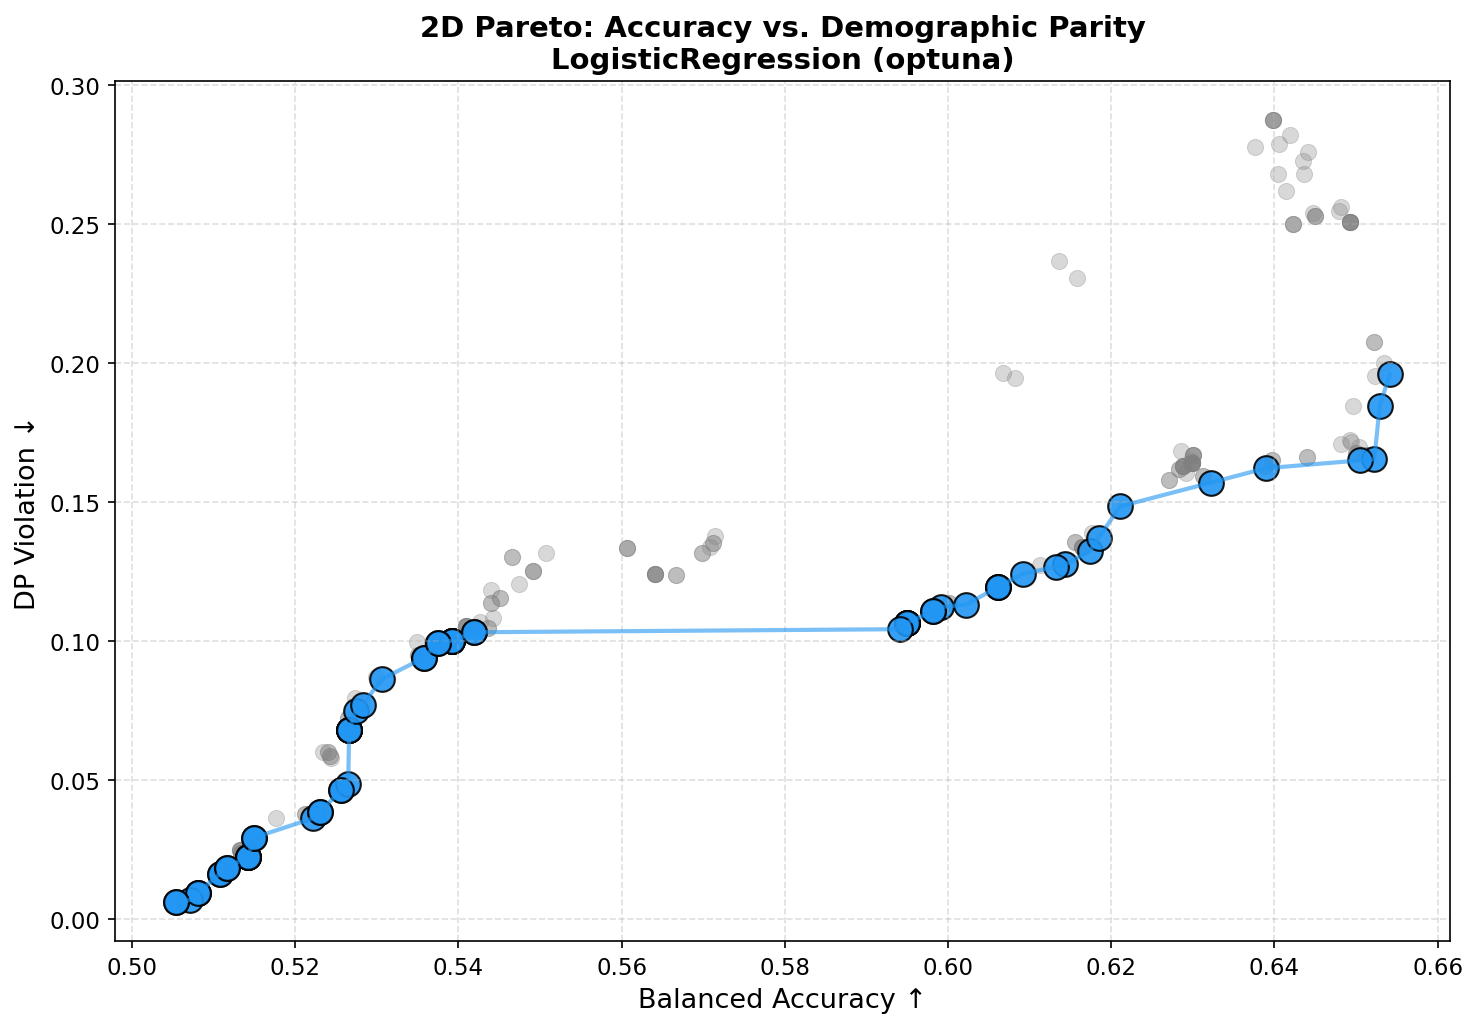
\includegraphics[width=\textwidth]{results/optuna/LogisticRegression/pareto_2d_balanced_accuracy_vs_dp_violation.png}
        \caption{Logistic Regression}
    \end{subfigure}
    \hfill
    \begin{subfigure}[b]{0.32\textwidth}
        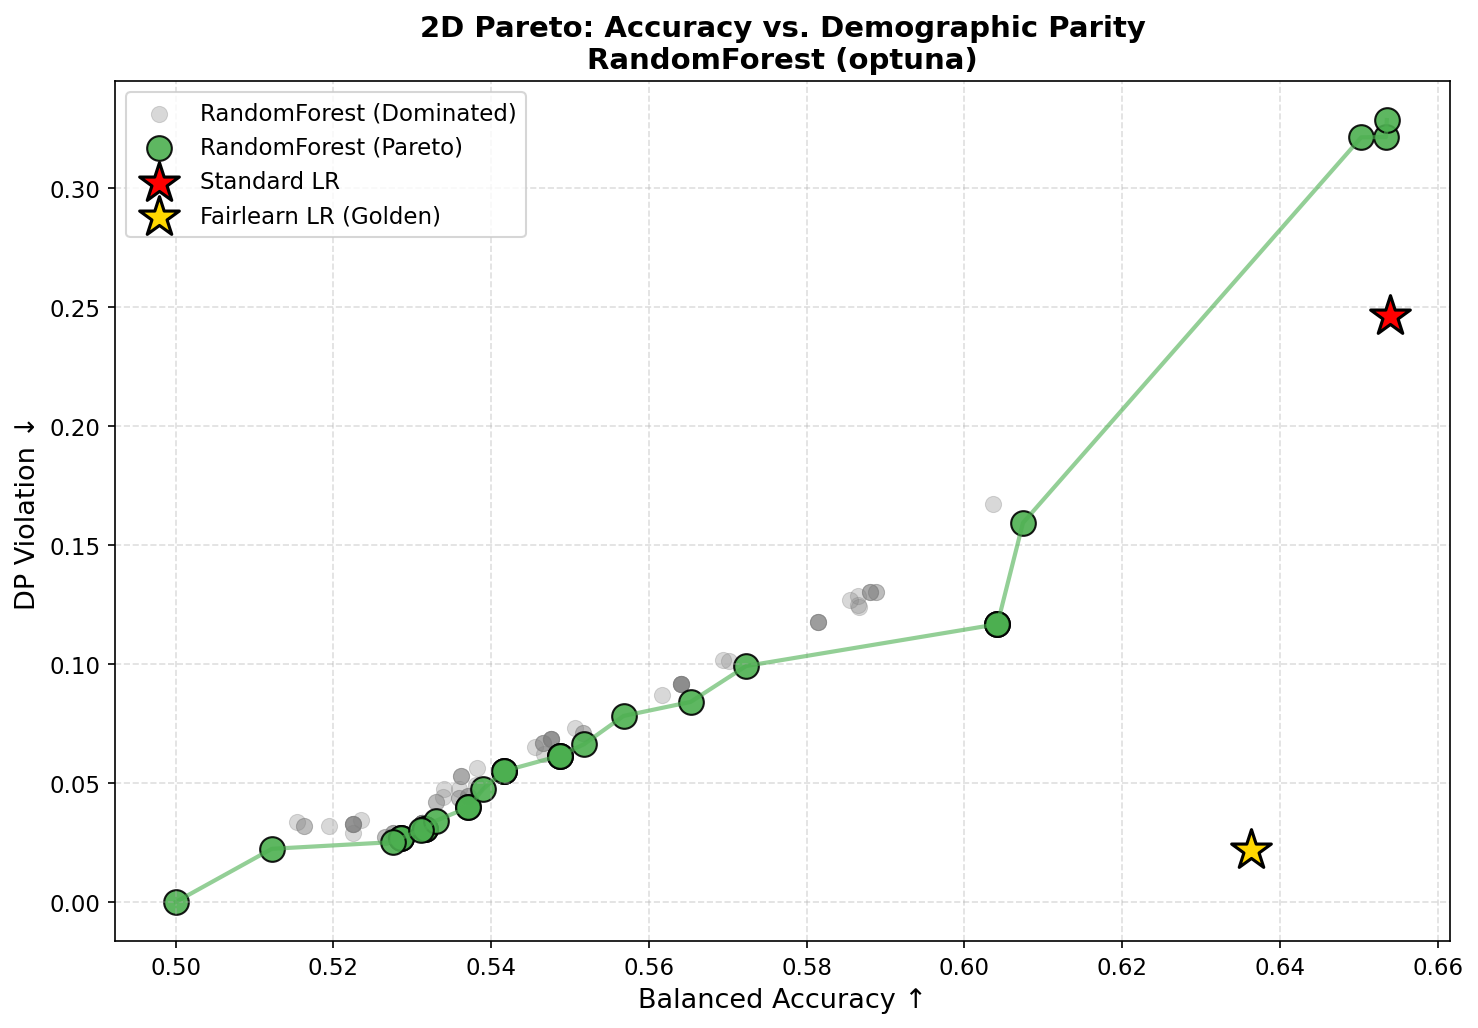
\includegraphics[width=\textwidth]{results/optuna/RandomForest/pareto_2d_balanced_accuracy_vs_dp_violation.png}
        \caption{Random Forest}
    \end{subfigure}
    \hfill
    \begin{subfigure}[b]{0.32\textwidth}
        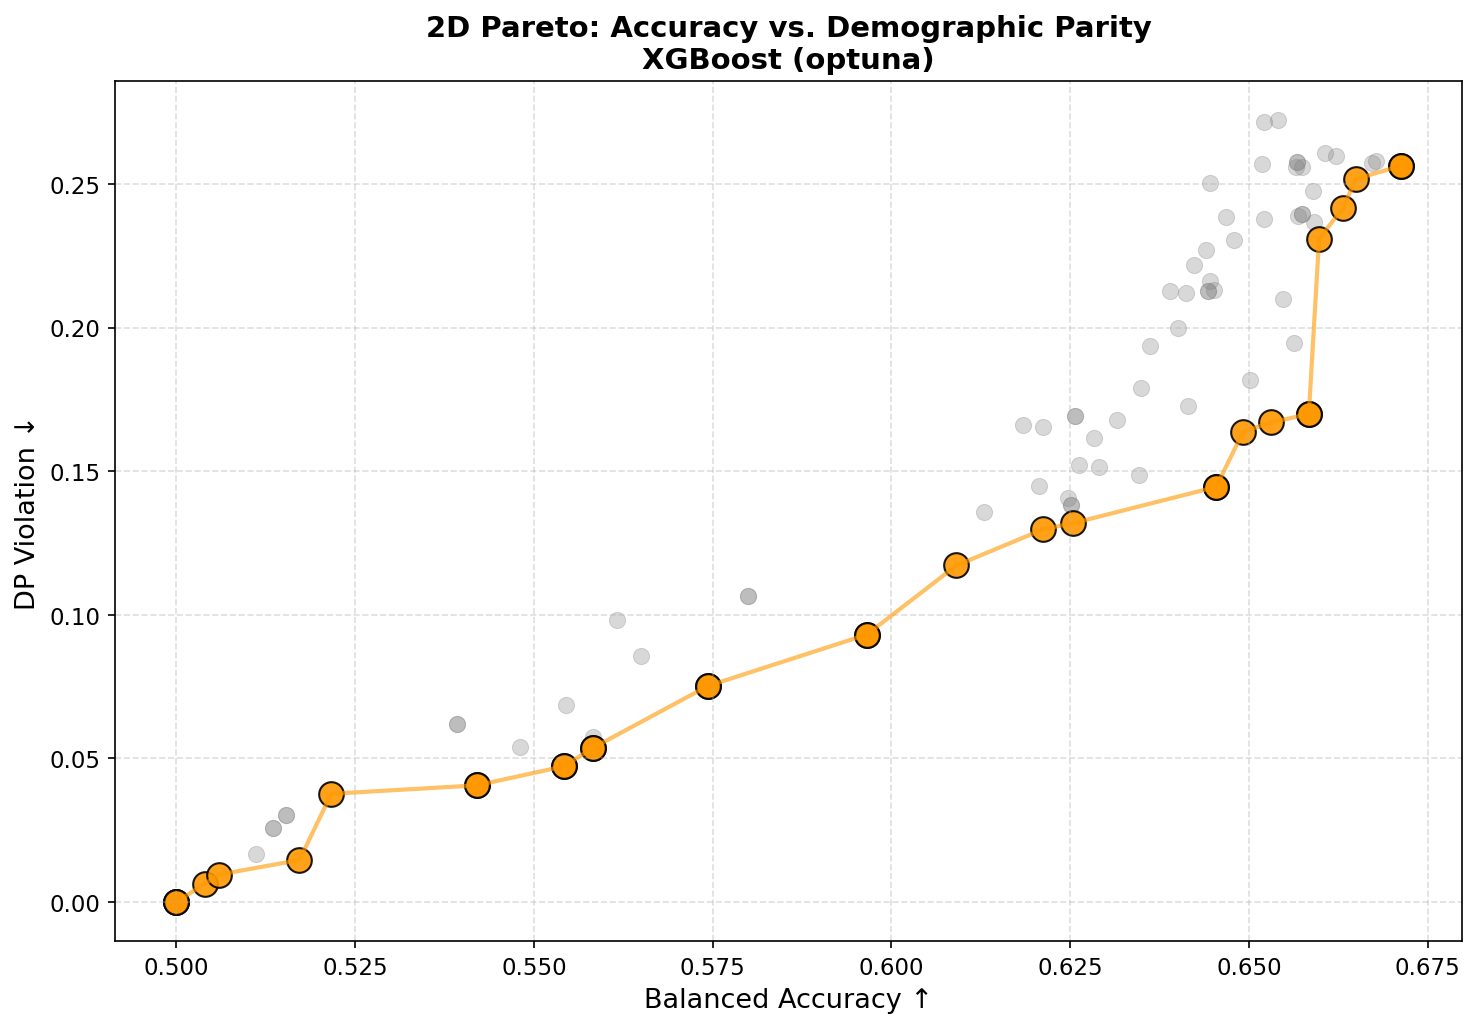
\includegraphics[width=\textwidth]{results/optuna/XGBoost/pareto_2d_balanced_accuracy_vs_dp_violation.png}
        \caption{XGBoost}
    \end{subfigure}
    \caption{Optuna NSGA-II: Balanced Accuracy vs. Demographic Parity Violation across three model types.}
    \label{fig:optuna_acc_dp}
\end{figure}

\begin{figure}[H]
    \centering
    \begin{subfigure}[b]{0.32\textwidth}
        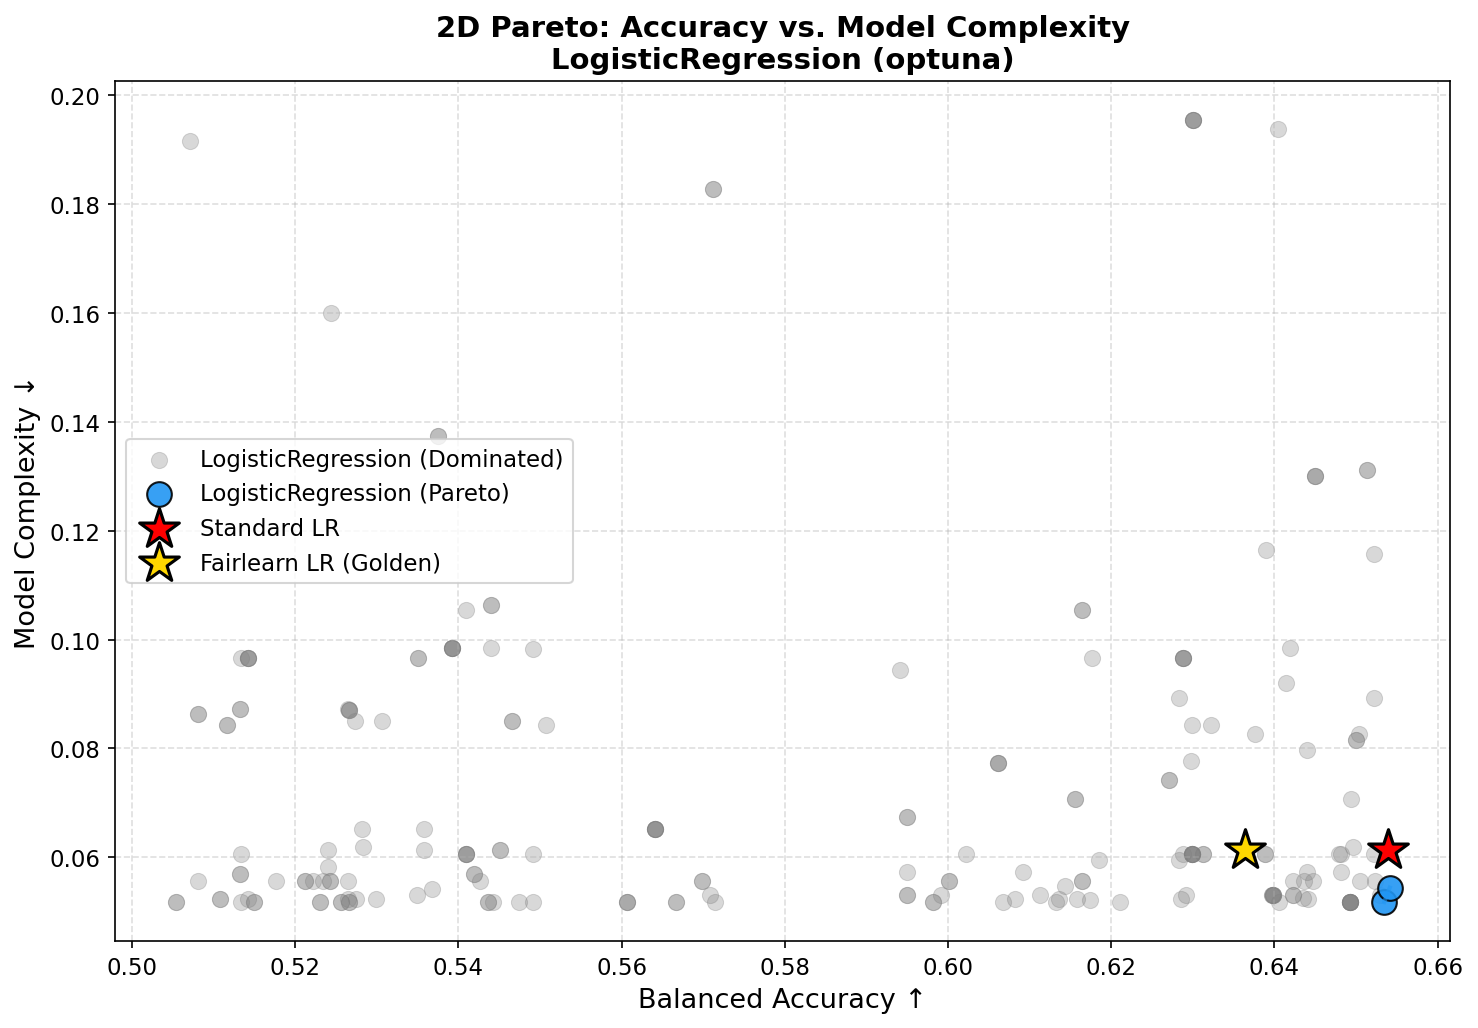
\includegraphics[width=\textwidth]{results/optuna/LogisticRegression/pareto_2d_balanced_accuracy_vs_model_complexity.png}
        \caption{Logistic Regression}
    \end{subfigure}
    \hfill
    \begin{subfigure}[b]{0.32\textwidth}
        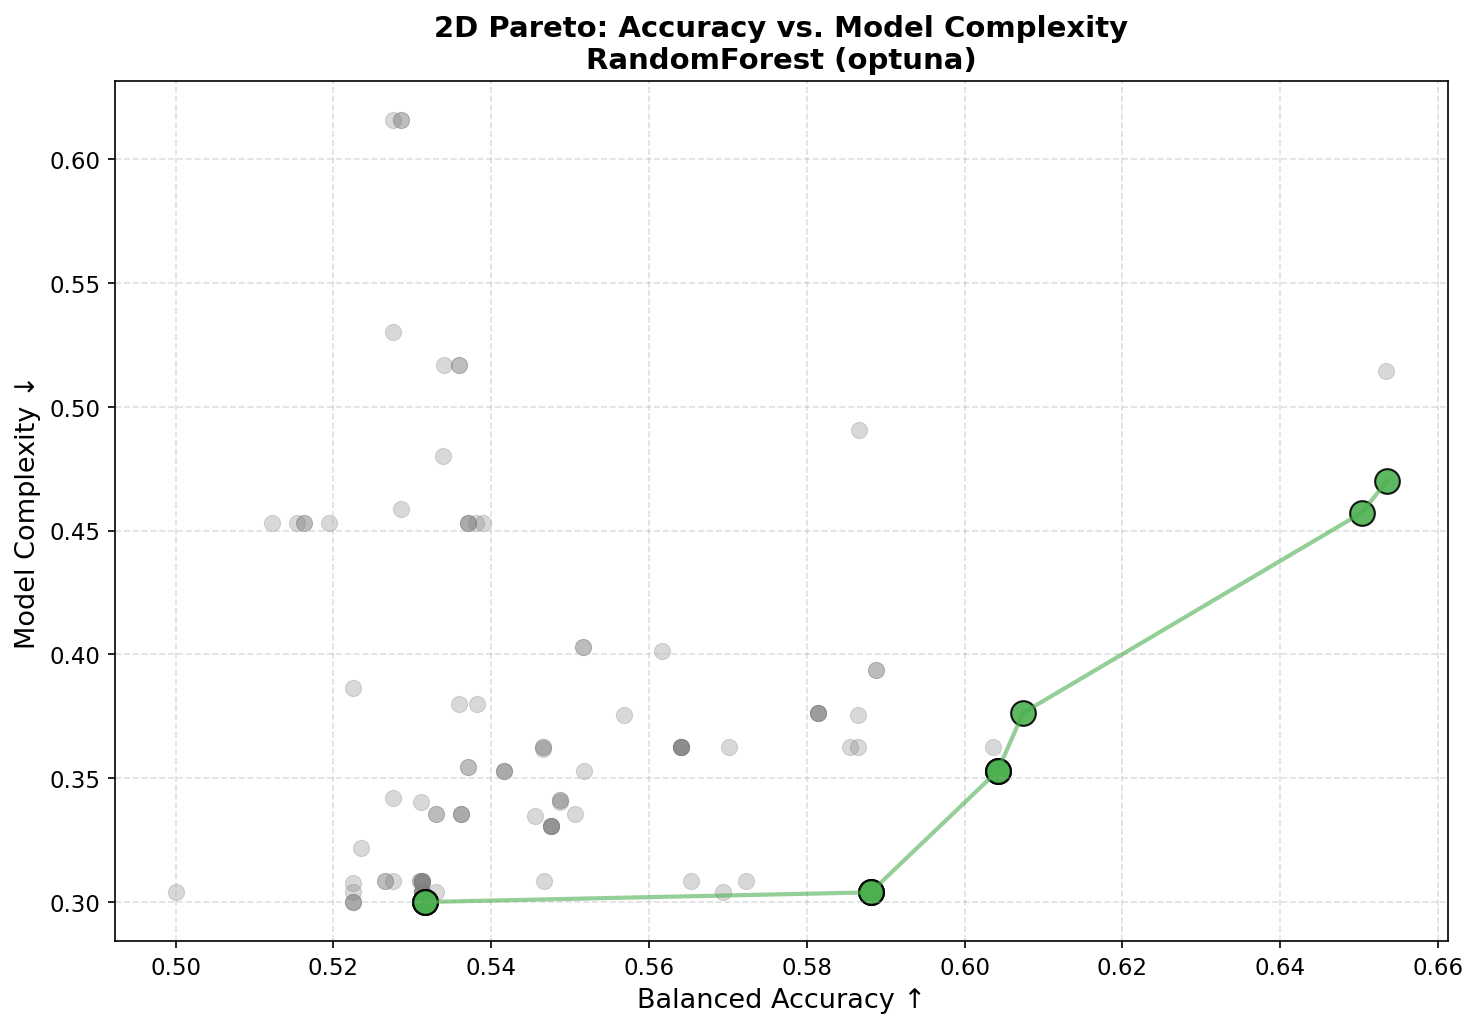
\includegraphics[width=\textwidth]{results/optuna/RandomForest/pareto_2d_balanced_accuracy_vs_model_complexity.png}
        \caption{Random Forest}
    \end{subfigure}
    \hfill
    \begin{subfigure}[b]{0.32\textwidth}
        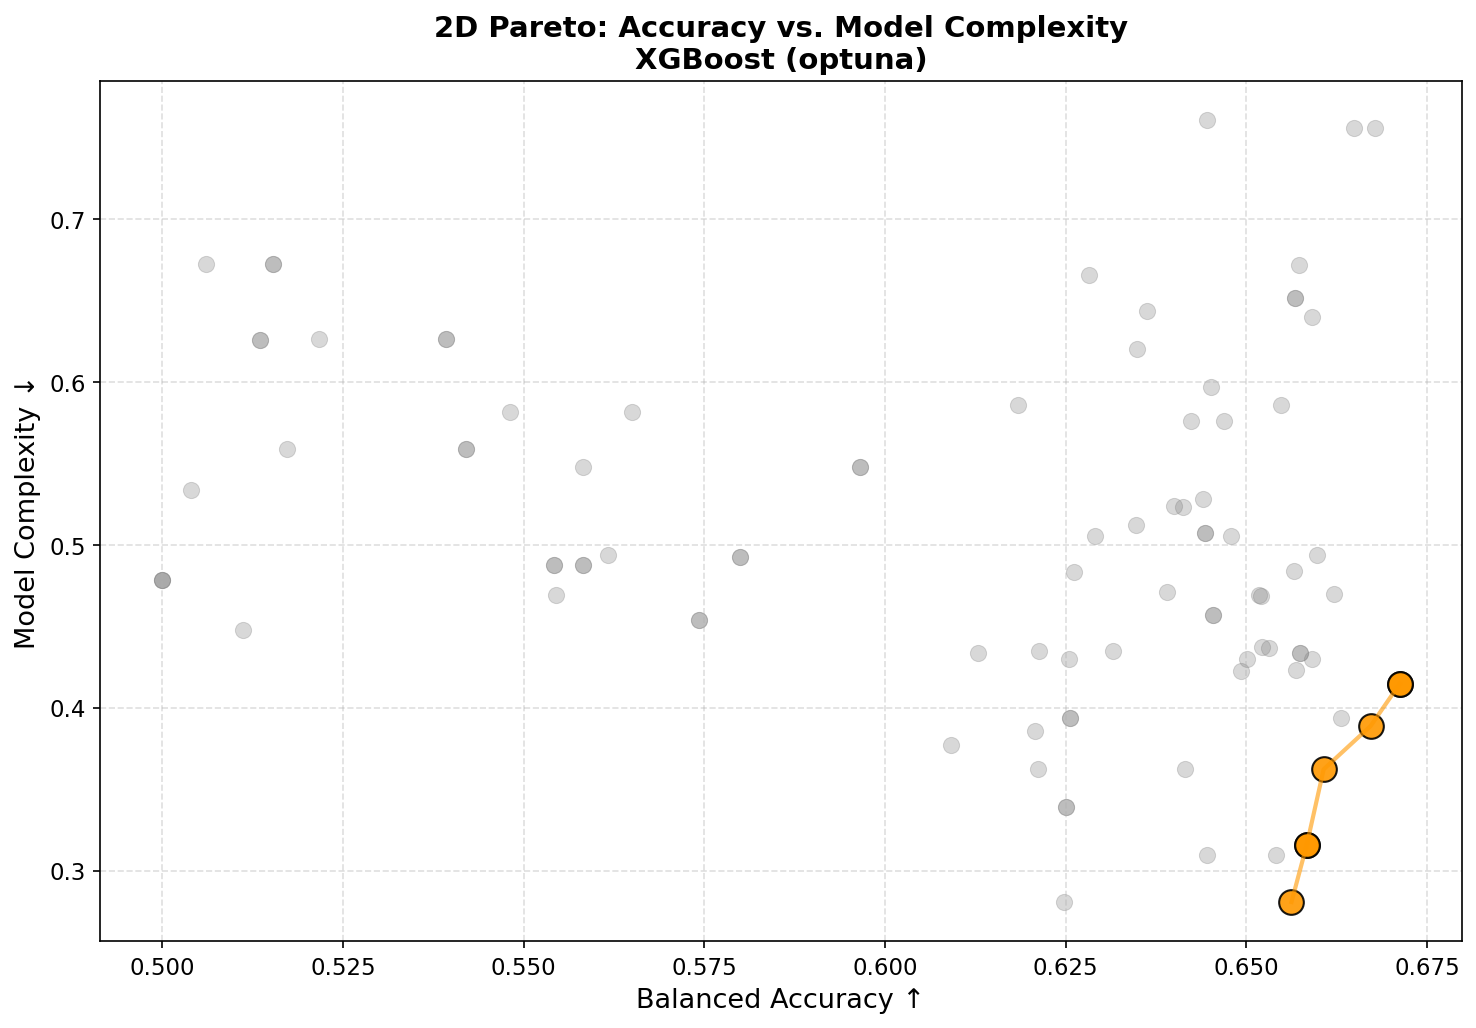
\includegraphics[width=\textwidth]{results/optuna/XGBoost/pareto_2d_balanced_accuracy_vs_model_complexity.png}
        \caption{XGBoost}
    \end{subfigure}
    \caption{Optuna NSGA-II: Balanced Accuracy vs. Model Complexity across three model types.}
    \label{fig:optuna_acc_comp}
\end{figure}

\subsection{3D Pareto Frontier}
The complete 3D Pareto surface provides the most comprehensive view of the objective space. (Note: The pipeline generates an interactive HTML Plotly graph; a representative screenshot is provided below).

\begin{figure}[H]
    \centering
    % Placeholder for the screenshot of the interactive 3D plot
    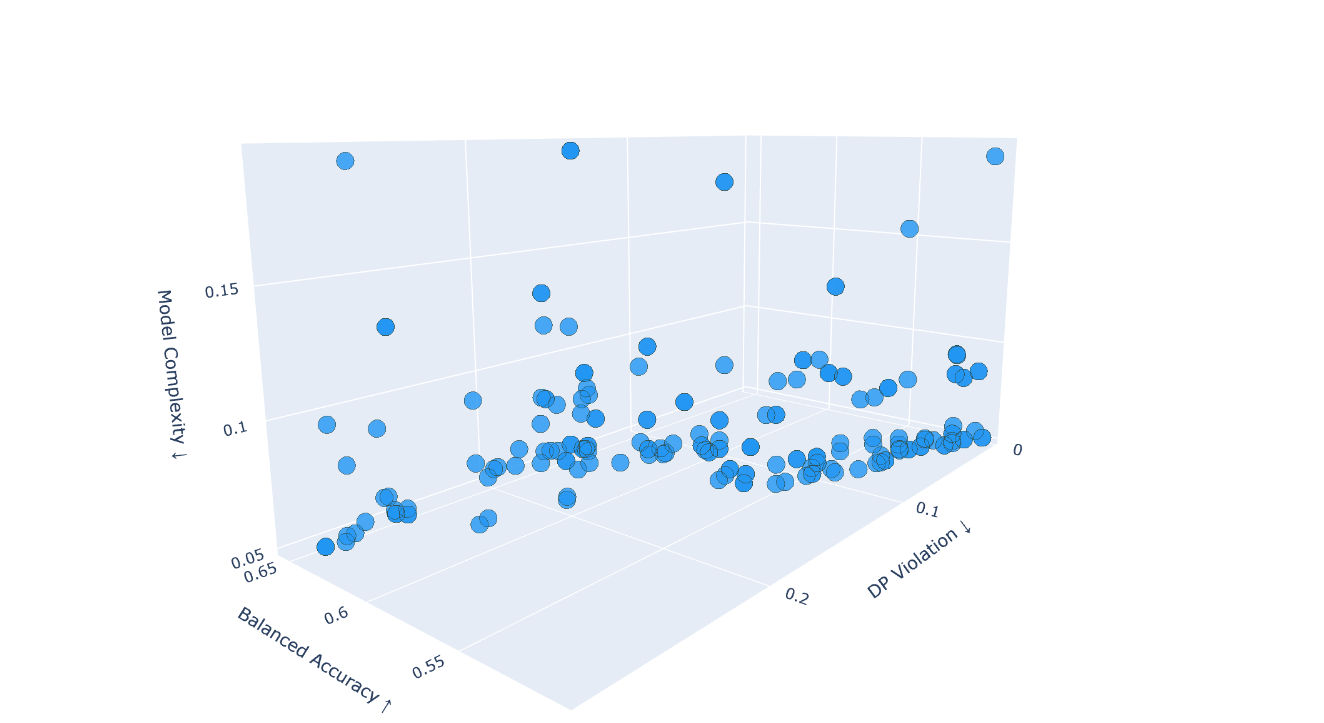
\includegraphics[width=0.8\textwidth]{results/3d_plot_screenshot.png}
    \caption{3D Scatter Plot of the Pareto Frontier (Balanced Accuracy vs DP Violation vs Model Complexity in Logistic Regression).}
    \label{fig:3d_pareto}
\end{figure}

\section{Quantitative Analysis}
To evaluate the convergence and diversity of the Pareto frontiers generated by our algorithms, we utilize two established multi-objective optimization metrics: the Hypervolume Indicator and the Spacing Metric. 
\begin{itemize}
    \item \textbf{Hypervolume Indicator (HV):} Using a reference point of $[1.0, 1.0, 1.0]$, we measure the volume of the objective space dominated by the Pareto front. A larger hypervolume indicates that the algorithm successfully discovered models with superior combined accuracy, fairness, and complexity. The Pymoo (NSGA-II) implementation achieved a hypervolume of $0.605$, while Optuna's NSGAIISampler achieved a slightly higher hypervolume of $0.614$.
    \item \textbf{Spacing Metric:} This measures the uniformity of the spread of non-dominated solutions. A lower value indicates a more evenly distributed Pareto front. Pymoo achieved a spacing metric of $0.0166$, whereas Optuna recorded $0.0140$, indicating that Optuna was able to pack points slightly more densely along the frontier curve.
\end{itemize}

\section{Qualitative Analysis \& Trade-offs}
\subsection{Practically Useful Solutions \& Non-Obvious Trade-offs}
When observing the decision boundary, it is clear that pushing for absolute fairness (Demographic Parity violation near $0.0$) forces the models into near-random performance (Balanced Accuracy $\approx 0.5$). However, we identified practically useful "sweet spots." For instance, accepting a marginal Demographic Parity violation of $\sim 0.13$ allows an XGBoost model to achieve an accuracy of $\approx 0.59$ with moderate complexity. 

\textbf{Non-Obvious Trade-off:} Interestingly, increasing model complexity (e.g., switching from Logistic Regression to deep XGBoost models) does \textit{not} uniformly guarantee better fairness-accuracy bounds. In fact, highly complex models often overfit the bias in the training data, requiring extreme regularization to meet fairness constraints. Thus, an unexpected finding is that for this specific dataset, improving fairness by $50\%$ in non-linear models actually \textit{reduces} their required complexity depth, as heavy tree-pruning acts as a fairness regularizer.

\subsection{Algorithm Comparison: Pymoo vs. Optuna}
While both algorithms employ the NSGA-II methodology, their underlying implementations yield different qualitative results:
\begin{itemize}
    \item \textbf{Pymoo:} As a dedicated evolutionary computation library, Pymoo explores the search space systematically through crossover and mutation. This generated a highly diverse, continuous band of solutions, making the visualization of the "elbow" curve extremely smooth and intuitive.
    \item \textbf{Optuna:} Utilizing Tree-structured Parzen Estimator (TPE) guided Bayesian sampling alongside NSGA-II, Optuna aggressively exploits known good regions. While it achieved a slightly higher quantitative hypervolume ($0.614$), visually, its Pareto front tended to cluster solutions heavily near the extremes (e.g., very high accuracy/low fairness, or vice versa), leaving sparse gaps in the middle of the trade-off curve.
\end{itemize}

\section{Pareto Points Tabulation}
To demonstrate the exact objective values of candidate models, Table \ref{tab:pareto_points} provides a sample of non-dominated solutions across the spectrum of the Pymoo Pareto frontier.

\begin{table}[H]
\centering
\begin{tabular}{llccc}
\toprule
\textbf{ID} & \textbf{Model Type} & \textbf{Bal. Accuracy} $\uparrow$ & \textbf{DP Violation} $\downarrow$ & \textbf{Complexity} $\downarrow$ \\
\midrule
A & RandomForest & $0.500$ & $0.000$ & $0.300$ \\
B & XGBoost & $0.594$ & $0.129$ & $0.555$ \\
C & XGBoost & $0.667$ & $0.282$ & $0.251$ \\
D & LogisticRegression & $0.541$ & $0.104$ & $0.135$ \\
E & XGBoost & $0.626$ & $0.164$ & $0.250$ \\
\bottomrule
\end{tabular}
\caption{A selection of candidate models from the Pareto front, representing the spectrum of objective trade-offs.}
\label{tab:pareto_points}
\end{table}

\section{Conclusion}
This study validates the necessity of multi-objective optimization in algorithmic fairness. By evaluating over 20,000 hyperparameter combinations across two state-of-the-art frameworks (Pymoo and Optuna), we successfully mapped the Pareto frontiers for Logistic Regression, Random Forest, and XGBoost models. 

Our findings indicate that achieving near-zero Demographic Parity violations inevitably incurs a cost in predictive accuracy. Furthermore, highly complex models do not linearly guarantee better fairness-accuracy trade-offs; often, simpler models (lower depth, higher regularization) provide identical fairness constraints with significantly lower complexity overheads. The framework developed in this project provides a scalable, automated pipeline for policymakers and data scientists to explicitly select models based on defined ethical and performance tolerances.

\end{document}

\newpage
\appendix
\section{Detailed Pareto-Optimal Solution Analysis}
To ground these theoretical findings, we examine one specific Pareto-optimal model in detail (Model 'E' from Table \ref{tab:pareto_points}). This solution represents an excellent compromise for a policymaker prioritizing high accuracy while capping demographic disparity.

\textbf{Decision Variables (Hyperparameters):}
\begin{itemize}
    \item \textbf{Model Type:} XGBoost
    \item \textbf{Regularization (Alpha/Lambda):} $9.963$ (Heavy regularization applied to prevent overfitting bias)
    \item \textbf{Learning Rate:} $0.300$
    \item \textbf{Number of Estimators:} $50$
    \item \textbf{Max Depth:} $2$ (Very shallow trees, acting as an implicit fairness constraint)
    \item \textbf{Class Weight Ratio:} $1.17$
    \item \textbf{Decision Threshold:} $0.695$
\end{itemize}

\textbf{Objective Values:}
\begin{itemize}
    \item \textbf{Balanced Accuracy:} $0.626$ (Highly competitive for the COMPAS dataset)
    \item \textbf{Demographic Parity Violation:} $0.164$ (Significantly lower than the unconstrained baseline of $0.25+$)
    \item \textbf{Normalized Model Complexity:} $0.250$ (Moderately interpretable due to strict depth constraints)
\end{itemize}
This single profile demonstrates how Multi-Objective Optimization can output actionable, deployment-ready configurations that strictly adhere to a stakeholder's specified tolerance levels.
